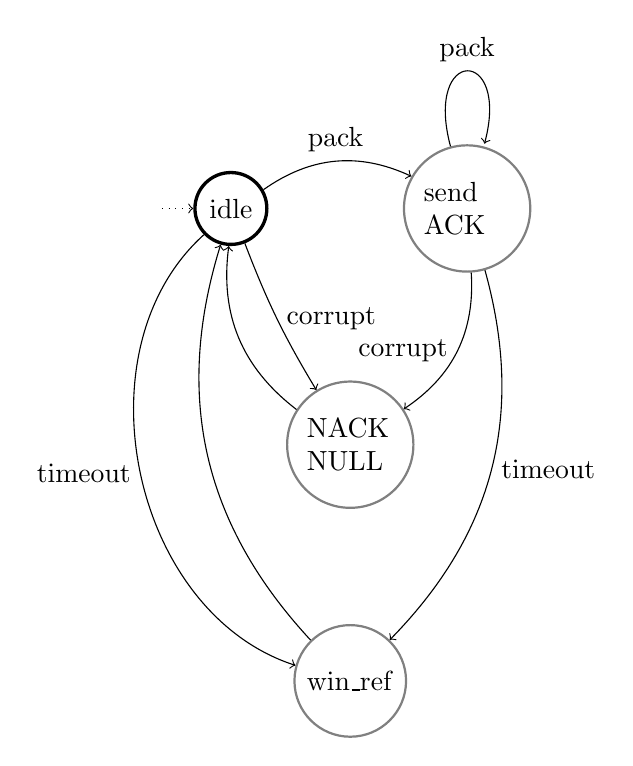
\begin{tikzpicture}
[
init/.style={circle, draw=black!100, very thick, minimum size=7mm,node distance=1cm},
state_split/.style={circle split, draw=gray!100, thick, minimum size=7mm,node distance=3cm,inner sep=0},
state/.style={circle, draw=gray!100, thick, minimum size=7mm,node distance=3cm,text width=11mm},
final/.style={circle, draw=black!60,  ultra thick, minimum size=10mm,node distance=23mm}
]
%Nodes
\node[init]     (start)                         {idle};
\node           (init)          [left of=start]     {};
\node[state]    (ack)          [right of=start]    {send ACK};
\node[state]    (nack)         [below of=start, right=7mm]    {NACK NULL};
%\node[state]    (wref)         [below of=nack]    {win_ref};
\node[state]    (wref)          [below of=nack]      {win\_ref};

%Lines
%\draw[->] (start.east) -- (synx.west);
%\draw[->] (synx.east) -- (end.west);
%\path[->] (start)  edge [loop above] node {a} (start); 
\draw[dotted, ->] (init.east) -- (start.west);
\path[->] 

(start) edge[bend left]                   node[above]             {pack}      (ack)
(start) edge [bend right=60]        node[left]             {timeout}   (wref)
(ack)   edge[loop above]        node[above]             {pack}      (ack)
(ack)   edge [bend left]        node[left]              {corrupt}   (nack)
(start) edge [bend right=5]        node[right]              {corrupt}   (nack)
(nack)  edge [bend left]        node                    {}          (start)
(ack)   edge [bend left]        node[right]             {timeout}   (wref)
(wref)  edge [bend left]        node                    {}          (start);





\end{tikzpicture}